
	\chapter{Der kosmische Mikrowellenhintergrund\label{chapter:thema}}
	\lhead{Der kosmische Mikrowellenhintergrund}
	\begin{refsection}
		\chapterauthor{Hansruedi Patzen und Nico Vinzens}
		
		\printbibliography[heading=subbibliography]
	\end{refsection}
	\section{Einleitung}
	Ähnlich wie der Lebensraum der Fische auf das Wasser begrenzt ist, so ist unser Lebensraum begrenzt auf das Universum.
	Weiss ein Fisch, wie das Meer von unserem Blickpunkt aus aussieht?
	Wahrscheinlich nicht, wieso sollte ihn das auch interessieren?
	Da wir aber keine Fische sind, ist es nur natürlich sich zu fragen, wie das Universum von Aussen betrachtet, aussieht.
	Um die Frage nach der Form des Universums beantworten zu können, werden wir uns im folgenden Kapitel mit dem kosmischen Mikrowellenhintergrund befassen.
	
	\subsection{Der komische Mikrowellenhintergrund}
	Glaubt man der Theorie des Big-Bang, (was wir im folgenden tun wollen) so waren der Druck und die Temperaturen in den ersten ca. 300'000 Jahren nach dem Big-Bang so, dass Atome nicht existieren konnten. Die gesamte Masse bestand stattdessen aus ionisiertem Plasma, welches sehr effizient darin war, Strahlung zu zerstreuen.
	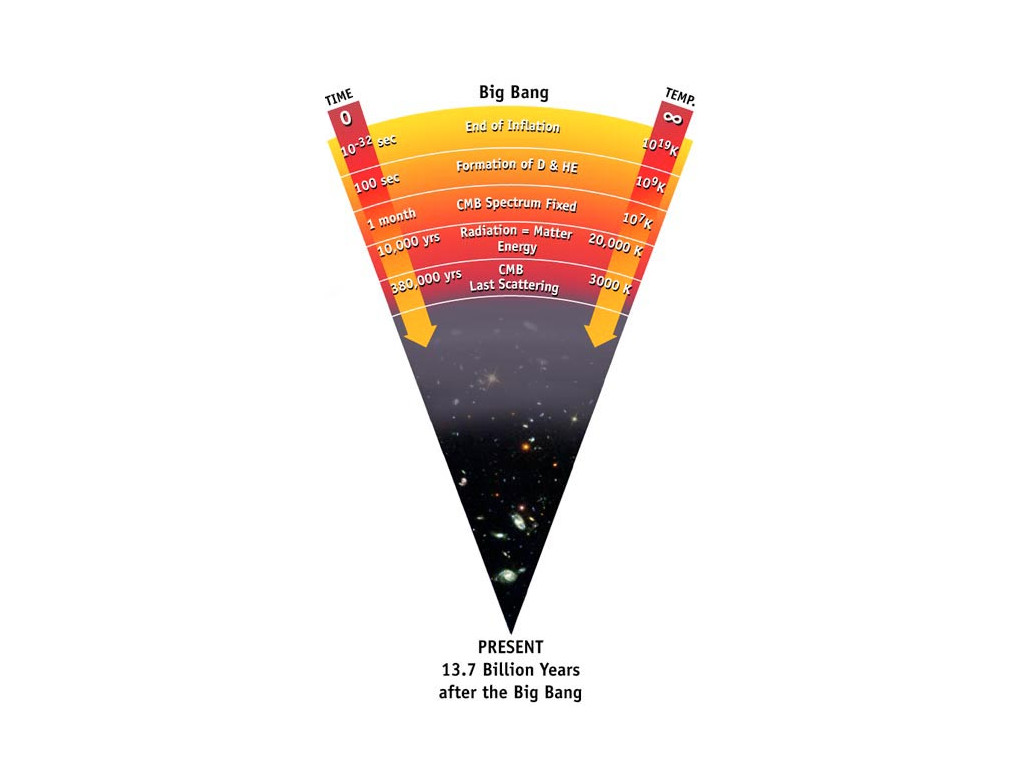
\includegraphics[scale=1]{images/radiation_scattering.png}
	\ref{CMB_intro}
	
	\subsection{Die Formen des Universums}
	Viele schlaue Köpfe haben sich bereits Gedanken darüber gemacht, welche Form das Unviersum haben könnte. Der Schlüssel zur Beantwortung dieser Frage ist in der Geometrie zu finden:
	\begin{itemize}
		\item Das Universum könnte positiv gekrümmt sein, wie eine Kugel.
		Zwei parallele Linien auf der Kugeloberfläche kreuzen sich und die Winkelsumme eines Dreiecks ist grösser als 360 Grad.
		\item Das Universum könnte negativ gekrümmt sein, wie ein Sattel.
		Zwei parallele Linien weichen immer stärker voneinander ab und die Winkelsumme eines Dreiecks ist kleiner als 360 Grad.
		\item Das Universum könnte flach sein, wie ein Blatt Papier.
		Zwei parallele Linien berühren sich nie und die Winkelsumme eines Dreiecks beträgt 360 Grad.
	\end{itemize}
	Wie kann diese Information genutzt werden, um die Form des Universums zu erklären?
	Wie wir bereits wissen, ist die kosmische Mikrowellenhintergrundstrahlung etwa 380'000 Jahre nach dem Urknall entstanden und ist heute noch erkennbar. 
	
